\documentclass[1p]{elsarticle_modified}
%\bibliographystyle{elsarticle-num}

%\usepackage[colorlinks]{hyperref}
%\usepackage{abbrmath_seonhwa} %\Abb, \Ascr, \Acal ,\Abf, \Afrak
\usepackage{amsfonts}
\usepackage{amssymb}
\usepackage{amsmath}
\usepackage{amsthm}
\usepackage{scalefnt}
\usepackage{amsbsy}
\usepackage{kotex}
\usepackage{caption}
\usepackage{subfig}
\usepackage{color}
\usepackage{graphicx}
\usepackage{xcolor} %% white, black, red, green, blue, cyan, magenta, yellow
\usepackage{float}
\usepackage{setspace}
\usepackage{hyperref}

\usepackage{tikz}
\usetikzlibrary{arrows}

\usepackage{multirow}
\usepackage{array} % fixed length table
\usepackage{hhline}

%%%%%%%%%%%%%%%%%%%%%
\makeatletter
\renewcommand*\env@matrix[1][\arraystretch]{%
	\edef\arraystretch{#1}%
	\hskip -\arraycolsep
	\let\@ifnextchar\new@ifnextchar
	\array{*\c@MaxMatrixCols c}}
\makeatother %https://tex.stackexchange.com/questions/14071/how-can-i-increase-the-line-spacing-in-a-matrix
%%%%%%%%%%%%%%%

\usepackage[normalem]{ulem}

\newcommand{\msout}[1]{\ifmmode\text{\sout{\ensuremath{#1}}}\else\sout{#1}\fi}
%SOURCE: \msout is \stkout macro in https://tex.stackexchange.com/questions/20609/strikeout-in-math-mode

\newcommand{\cancel}[1]{
	\ifmmode
	{\color{red}\msout{#1}}
	\else
	{\color{red}\sout{#1}}
	\fi
}

\newcommand{\add}[1]{
	{\color{blue}\uwave{#1}}
}

\newcommand{\replace}[2]{
	\ifmmode
	{\color{red}\msout{#1}}{\color{blue}\uwave{#2}}
	\else
	{\color{red}\sout{#1}}{\color{blue}\uwave{#2}}
	\fi
}

\newcommand{\Sol}{\mathcal{S}} %segment
\newcommand{\D}{D} %diagram
\newcommand{\A}{\mathcal{A}} %arc


%%%%%%%%%%%%%%%%%%%%%%%%%%%%%5 test

\def\sl{\operatorname{\textup{SL}}(2,\Cbb)}
\def\psl{\operatorname{\textup{PSL}}(2,\Cbb)}
\def\quan{\mkern 1mu \triangleright \mkern 1mu}

\theoremstyle{definition}
\newtheorem{thm}{Theorem}[section]
\newtheorem{prop}[thm]{Proposition}
\newtheorem{lem}[thm]{Lemma}
\newtheorem{ques}[thm]{Question}
\newtheorem{cor}[thm]{Corollary}
\newtheorem{defn}[thm]{Definition}
\newtheorem{exam}[thm]{Example}
\newtheorem{rmk}[thm]{Remark}
\newtheorem{alg}[thm]{Algorithm}

\newcommand{\I}{\sqrt{-1}}
\begin{document}

%\begin{frontmatter}
%
%\title{Boundary parabolic representations of knots up to 8 crossings}
%
%%% Group authors per affiliation:
%\author{Yunhi Cho} 
%\address{Department of Mathematics, University of Seoul, Seoul, Korea}
%\ead{yhcho@uos.ac.kr}
%
%
%\author{Seonhwa Kim} %\fnref{s_kim}}
%\address{Center for Geometry and Physics, Institute for Basic Science, Pohang, 37673, Korea}
%\ead{ryeona17@ibs.re.kr}
%
%\author{Hyuk Kim}
%\address{Department of Mathematical Sciences, Seoul National University, Seoul 08826, Korea}
%\ead{hyukkim@snu.ac.kr}
%
%\author{Seokbeom Yoon}
%\address{Department of Mathematical Sciences, Seoul National University, Seoul, 08826,  Korea}
%\ead{sbyoon15@snu.ac.kr}
%
%\begin{abstract}
%We find all boundary parabolic representation of knots up to 8 crossings.
%
%\end{abstract}
%\begin{keyword}
%    \MSC[2010] 57M25 
%\end{keyword}
%
%\end{frontmatter}

%\linenumbers
%\tableofcontents
%
\newcommand\colored[1]{\textcolor{white}{\rule[-0.35ex]{0.8em}{1.4ex}}\kern-0.8em\color{red} #1}%
%\newcommand\colored[1]{\textcolor{white}{ #1}\kern-2.17ex	\textcolor{white}{ #1}\kern-1.81ex	\textcolor{white}{ #1}\kern-2.15ex\color{red}#1	}

{\Large $\underline{12n_{0749}~(K12n_{0749})}$}

\setlength{\tabcolsep}{10pt}
\renewcommand{\arraystretch}{1.6}
\vspace{1cm}\begin{tabular}{m{100pt}>{\centering\arraybackslash}m{274pt}}
\multirow{5}{120pt}{
	\centering
	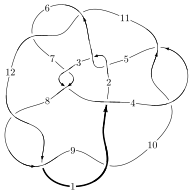
\includegraphics[width=112pt]{../../../GIT/diagram.site/Diagrams/png/2838_12n_0749.png}\\
\ \ \ A knot diagram\footnotemark}&
\allowdisplaybreaks
\textbf{Linearized knot diagam} \\
\cline{2-2}
 &
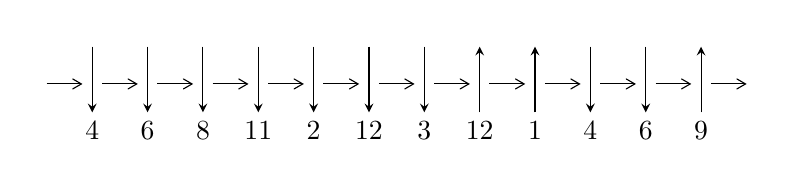
\begin{tikzpicture}[x=20pt, y=17pt]
	% nodes
	\node (C0) at (0, 0) {};
	\node (C1) at (1, 0) {};
	\node (C1U) at (1, +1) {};
	\node (C1D) at (1, -1) {4};

	\node (C2) at (2, 0) {};
	\node (C2U) at (2, +1) {};
	\node (C2D) at (2, -1) {6};

	\node (C3) at (3, 0) {};
	\node (C3U) at (3, +1) {};
	\node (C3D) at (3, -1) {8};

	\node (C4) at (4, 0) {};
	\node (C4U) at (4, +1) {};
	\node (C4D) at (4, -1) {11};

	\node (C5) at (5, 0) {};
	\node (C5U) at (5, +1) {};
	\node (C5D) at (5, -1) {2};

	\node (C6) at (6, 0) {};
	\node (C6U) at (6, +1) {};
	\node (C6D) at (6, -1) {12};

	\node (C7) at (7, 0) {};
	\node (C7U) at (7, +1) {};
	\node (C7D) at (7, -1) {3};

	\node (C8) at (8, 0) {};
	\node (C8U) at (8, +1) {};
	\node (C8D) at (8, -1) {12};

	\node (C9) at (9, 0) {};
	\node (C9U) at (9, +1) {};
	\node (C9D) at (9, -1) {1};

	\node (C10) at (10, 0) {};
	\node (C10U) at (10, +1) {};
	\node (C10D) at (10, -1) {4};

	\node (C11) at (11, 0) {};
	\node (C11U) at (11, +1) {};
	\node (C11D) at (11, -1) {6};

	\node (C12) at (12, 0) {};
	\node (C12U) at (12, +1) {};
	\node (C12D) at (12, -1) {9};
	\node (C13) at (13, 0) {};

	% arrows
	\draw[->,>={angle 60}]
	(C0) edge (C1) (C1) edge (C2) (C2) edge (C3) (C3) edge (C4) (C4) edge (C5) (C5) edge (C6) (C6) edge (C7) (C7) edge (C8) (C8) edge (C9) (C9) edge (C10) (C10) edge (C11) (C11) edge (C12) (C12) edge (C13) ;	\draw[->,>=stealth]
	(C1U) edge (C1D) (C2U) edge (C2D) (C3U) edge (C3D) (C4U) edge (C4D) (C5U) edge (C5D) (C6U) edge (C6D) (C7U) edge (C7D) (C8D) edge (C8U) (C9D) edge (C9U) (C10U) edge (C10D) (C11U) edge (C11D) (C12D) edge (C12U) ;
	\end{tikzpicture} \\
\hhline{~~} \\& 
\textbf{Solving Sequence} \\ \cline{2-2} 
 &
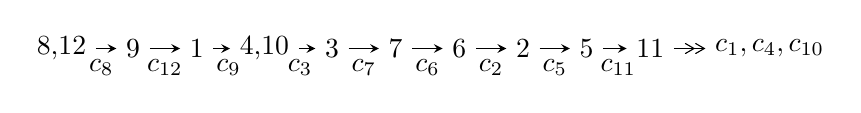
\begin{tikzpicture}[x=23pt, y=7pt]
	% node
	\node (A0) at (-1/8, 0) {8,12};
	\node (A1) at (1, 0) {9};
	\node (A2) at (2, 0) {1};
	\node (A3) at (49/16, 0) {4,10};
	\node (A4) at (33/8, 0) {3};
	\node (A5) at (41/8, 0) {7};
	\node (A6) at (49/8, 0) {6};
	\node (A7) at (57/8, 0) {2};
	\node (A8) at (65/8, 0) {5};
	\node (A9) at (73/8, 0) {11};
	\node (C1) at (1/2, -1) {$c_{8}$};
	\node (C2) at (3/2, -1) {$c_{12}$};
	\node (C3) at (5/2, -1) {$c_{9}$};
	\node (C4) at (29/8, -1) {$c_{3}$};
	\node (C5) at (37/8, -1) {$c_{7}$};
	\node (C6) at (45/8, -1) {$c_{6}$};
	\node (C7) at (53/8, -1) {$c_{2}$};
	\node (C8) at (61/8, -1) {$c_{5}$};
	\node (C9) at (69/8, -1) {$c_{11}$};
	\node (A10) at (11, 0) {$c_{1},c_{4},c_{10}$};

	% edge
	\draw[->,>=stealth]	
	(A0) edge (A1) (A1) edge (A2) (A2) edge (A3) (A3) edge (A4) (A4) edge (A5) (A5) edge (A6) (A6) edge (A7) (A7) edge (A8) (A8) edge (A9) ;
	\draw[->>,>={angle 60}]	
	(A9) edge (A10);
\end{tikzpicture} \\ 

\end{tabular} \\

\footnotetext{
The image of knot diagram is generated by the software ``\textbf{Draw programme}" developed by Andrew Bartholomew(\url{http://www.layer8.co.uk/maths/draw/index.htm\#Running-draw}), where we modified some parts for our purpose(\url{https://github.com/CATsTAILs/LinksPainter}).
}\phantom \\ \newline 
\centering \textbf{Ideals for irreducible components\footnotemark of $X_{\text{par}}$} 
 
\begin{align*}
I^u_{1}&=\langle 
u^7+u^6-5 u^5-5 u^4+6 u^3+8 u^2+b+u-1,\;- u^7- u^6+5 u^5+5 u^4-6 u^3-8 u^2+a- u+2,\\
\phantom{I^u_{1}}&\phantom{= \langle  }u^9+3 u^8-3 u^7-15 u^6-3 u^5+22 u^4+15 u^3-5 u^2-5 u+1\rangle \\
I^u_{2}&=\langle 
- u^4+u^3+3 u^2+b- u-2,\;u^4- u^3-3 u^2+a+u+3,\;u^6-2 u^5-3 u^4+5 u^3+4 u^2-3 u-1\rangle \\
\\
\end{align*}
\raggedright * 2 irreducible components of $\dim_{\mathbb{C}}=0$, with total 15 representations.\\
\footnotetext{All coefficients of polynomials are rational numbers. But the coefficients are sometimes approximated in decimal forms when there is not enough margin.}
\newpage
\renewcommand{\arraystretch}{1}
\centering \section*{I. $I^u_{1}= \langle u^7+u^6-5 u^5-5 u^4+6 u^3+8 u^2+b+u-1,\;- u^7- u^6+5 u^5+5 u^4-6 u^3-8 u^2+a- u+2,\;u^9+3 u^8+\cdots-5 u+1 \rangle$}
\flushleft \textbf{(i) Arc colorings}\\
\begin{tabular}{m{7pt} m{180pt} m{7pt} m{180pt} }
\flushright $a_{8}=$&$\begin{pmatrix}1\\0\end{pmatrix}$ \\
\flushright $a_{12}=$&$\begin{pmatrix}0\\u\end{pmatrix}$ \\
\flushright $a_{9}=$&$\begin{pmatrix}1\\- u^2\end{pmatrix}$ \\
\flushright $a_{1}=$&$\begin{pmatrix}u\\- u^3+u\end{pmatrix}$ \\
\flushright $a_{4}=$&$\begin{pmatrix}u^7+u^6-5 u^5-5 u^4+6 u^3+8 u^2+u-2\\- u^7- u^6+5 u^5+5 u^4-6 u^3-8 u^2- u+1\end{pmatrix}$ \\
\flushright $a_{10}=$&$\begin{pmatrix}- u^2+1\\u^4-2 u^2\end{pmatrix}$ \\
\flushright $a_{3}=$&$\begin{pmatrix}-1\\- u^7- u^6+5 u^5+5 u^4-6 u^3-8 u^2- u+1\end{pmatrix}$ \\
\flushright $a_{7}=$&$\begin{pmatrix}- u^7- u^6+5 u^5+5 u^4-6 u^3-8 u^2- u+2\\u^8-6 u^6+12 u^4+3 u^3-9 u^2-5 u+1\end{pmatrix}$ \\
\flushright $a_{6}=$&$\begin{pmatrix}- u^7- u^6+5 u^5+5 u^4-6 u^3-8 u^2- u+2\\- u^8-2 u^7+4 u^6+9 u^5-2 u^4-11 u^3-6 u^2\end{pmatrix}$ \\
\flushright $a_{2}=$&$\begin{pmatrix}u^8+u^7-5 u^6-5 u^5+7 u^4+8 u^3- u^2-2 u\\-3 u^8-3 u^7+16 u^6+15 u^5-25 u^4-26 u^3+8 u^2+12 u-2\end{pmatrix}$ \\
\flushright $a_{5}=$&$\begin{pmatrix}7 u^8+7 u^7-37 u^6-33 u^5+56 u^4+54 u^3-17 u^2-22 u+6\\-2 u^8-3 u^7+11 u^6+13 u^5-17 u^4-19 u^3+5 u^2+8 u-2\end{pmatrix}$ \\
\flushright $a_{11}=$&$\begin{pmatrix}u^8+u^7-5 u^6-5 u^5+7 u^4+8 u^3-2 u^2-3 u+1\\-3 u^8-3 u^7+16 u^6+15 u^5-24 u^4-25 u^3+6 u^2+11 u-2\end{pmatrix}$\\&\end{tabular}
\flushleft \textbf{(ii) Obstruction class $= -1$}\\~\\
\flushleft \textbf{(iii) Cusp Shapes $= 3 u^8+11 u^7-6 u^6-54 u^5-23 u^4+73 u^3+62 u^2-4 u-17$}\\~\\
\newpage\renewcommand{\arraystretch}{1}
\flushleft \textbf{(iv) u-Polynomials at the component}\newline \\
\begin{tabular}{m{50pt}|m{274pt}}
Crossings & \hspace{64pt}u-Polynomials at each crossing \\
\hline $$\begin{aligned}c_{1},c_{4},c_{10}\end{aligned}$$&$\begin{aligned}
&u^9- u^8+18 u^7+15 u^6-15 u^5+3 u^4-13 u^3-4 u^2-2 u-1
\end{aligned}$\\
\hline $$\begin{aligned}c_{2},c_{5}\end{aligned}$$&$\begin{aligned}
&u^9+15 u^7-31 u^6+42 u^5-72 u^4+30 u^3+10 u^2-7 u+1
\end{aligned}$\\
\hline $$\begin{aligned}c_{3},c_{7}\end{aligned}$$&$\begin{aligned}
&u^9-9 u^8+38 u^7-94 u^6+144 u^5-132 u^4+57 u^3+8 u^2-20 u+8
\end{aligned}$\\
\hline $$\begin{aligned}c_{6},c_{11}\end{aligned}$$&$\begin{aligned}
&u^9+2 u^8+12 u^7+4 u^6+39 u^5+14 u^4+8 u^3+11 u^2- u-1
\end{aligned}$\\
\hline $$\begin{aligned}c_{8},c_{9},c_{12}\end{aligned}$$&$\begin{aligned}
&u^9-3 u^8-3 u^7+15 u^6-3 u^5-22 u^4+15 u^3+5 u^2-5 u-1
\end{aligned}$\\
\hline
\end{tabular}\\~\\
\newpage\renewcommand{\arraystretch}{1}
\flushleft \textbf{(v) Riley Polynomials at the component}\newline \\
\begin{tabular}{m{50pt}|m{274pt}}
Crossings & \hspace{64pt}Riley Polynomials at each crossing \\
\hline $$\begin{aligned}c_{1},c_{4},c_{10}\end{aligned}$$&$\begin{aligned}
&y^9+35 y^8+\cdots-4 y-1
\end{aligned}$\\
\hline $$\begin{aligned}c_{2},c_{5}\end{aligned}$$&$\begin{aligned}
&y^9+30 y^8+\cdots+29 y-1
\end{aligned}$\\
\hline $$\begin{aligned}c_{3},c_{7}\end{aligned}$$&$\begin{aligned}
&y^9-5 y^8+\cdots+272 y-64
\end{aligned}$\\
\hline $$\begin{aligned}c_{6},c_{11}\end{aligned}$$&$\begin{aligned}
&y^9+20 y^8+\cdots+23 y-1
\end{aligned}$\\
\hline $$\begin{aligned}c_{8},c_{9},c_{12}\end{aligned}$$&$\begin{aligned}
&y^9-15 y^8+\cdots+35 y-1
\end{aligned}$\\
\hline
\end{tabular}\\~\\
\newpage\flushleft \textbf{(vi) Complex Volumes and Cusp Shapes}
$$\begin{array}{c|c|c}  
\text{Solutions to }I^u_{1}& \I (\text{vol} + \sqrt{-1}CS) & \text{Cusp shape}\\
 \hline 
\begin{aligned}
u &= -0.803718 + 0.480044 I \\
a &= -0.545358 + 0.558768 I \\
b &= -0.454642 - 0.558768 I\end{aligned}
 & \phantom{-}1.43676 - 1.39156 I & -1.67156 + 5.14855 I \\ \hline\begin{aligned}
u &= -0.803718 - 0.480044 I \\
a &= -0.545358 - 0.558768 I \\
b &= -0.454642 + 0.558768 I\end{aligned}
 & \phantom{-}1.43676 + 1.39156 I & -1.67156 - 5.14855 I \\ \hline\begin{aligned}
u &= -1.39574\phantom{ +0.000000I} \\
a &= \phantom{-}0.458311\phantom{ +0.000000I} \\
b &= -1.45831\phantom{ +0.000000I}\end{aligned}
 & -1.87529\phantom{ +0.000000I} & -5.03640\phantom{ +0.000000I} \\ \hline\begin{aligned}
u &= \phantom{-}0.479009\phantom{ +0.000000I} \\
a &= \phantom{-}0.602594\phantom{ +0.000000I} \\
b &= -1.60259\phantom{ +0.000000I}\end{aligned}
 & -8.12479\phantom{ +0.000000I} & \phantom{-}0.759950\phantom{ +0.000000I} \\ \hline\begin{aligned}
u &= \phantom{-}1.56290 + 0.23534 I \\
a &= \phantom{-}0.115329 - 1.184520 I \\
b &= -1.11533 + 1.18452 I\end{aligned}
 & \phantom{-}9.69068 + 4.28297 I & -4.64998 - 2.95733 I \\ \hline\begin{aligned}
u &= \phantom{-}1.56290 - 0.23534 I \\
a &= \phantom{-}0.115329 + 1.184520 I \\
b &= -1.11533 - 1.18452 I\end{aligned}
 & \phantom{-}9.69068 - 4.28297 I & -4.64998 + 2.95733 I \\ \hline\begin{aligned}
u &= \phantom{-}0.189912\phantom{ +0.000000I} \\
a &= -1.48814\phantom{ +0.000000I} \\
b &= \phantom{-}0.488141\phantom{ +0.000000I}\end{aligned}
 & -0.677543\phantom{ +0.000000I} & -15.0670\phantom{ +0.000000I} \\ \hline\begin{aligned}
u &= -1.89577 + 0.05938 I \\
a &= \phantom{-}0.64365 + 1.55034 I \\
b &= -1.64365 - 1.55034 I\end{aligned}
 & -16.4807 - 5.9861 I & -4.50677 + 1.85792 I \\ \hline\begin{aligned}
u &= -1.89577 - 0.05938 I \\
a &= \phantom{-}0.64365 - 1.55034 I \\
b &= -1.64365 + 1.55034 I\end{aligned}
 & -16.4807 + 5.9861 I & -4.50677 - 1.85792 I\\
 \hline 
 \end{array}$$\newpage\newpage\renewcommand{\arraystretch}{1}
\centering \section*{II. $I^u_{2}= \langle - u^4+u^3+3 u^2+b- u-2,\;u^4- u^3-3 u^2+a+u+3,\;u^6-2 u^5-3 u^4+5 u^3+4 u^2-3 u-1 \rangle$}
\flushleft \textbf{(i) Arc colorings}\\
\begin{tabular}{m{7pt} m{180pt} m{7pt} m{180pt} }
\flushright $a_{8}=$&$\begin{pmatrix}1\\0\end{pmatrix}$ \\
\flushright $a_{12}=$&$\begin{pmatrix}0\\u\end{pmatrix}$ \\
\flushright $a_{9}=$&$\begin{pmatrix}1\\- u^2\end{pmatrix}$ \\
\flushright $a_{1}=$&$\begin{pmatrix}u\\- u^3+u\end{pmatrix}$ \\
\flushright $a_{4}=$&$\begin{pmatrix}- u^4+u^3+3 u^2- u-3\\u^4- u^3-3 u^2+u+2\end{pmatrix}$ \\
\flushright $a_{10}=$&$\begin{pmatrix}- u^2+1\\u^4-2 u^2\end{pmatrix}$ \\
\flushright $a_{3}=$&$\begin{pmatrix}-1\\u^4- u^3-3 u^2+u+2\end{pmatrix}$ \\
\flushright $a_{7}=$&$\begin{pmatrix}u^4- u^3-3 u^2+u+3\\u^5- u^4-3 u^3+2 u^2+2 u-2\end{pmatrix}$ \\
\flushright $a_{6}=$&$\begin{pmatrix}u^4- u^3-3 u^2+u+3\\- u^4+u^3+3 u^2- u-3\end{pmatrix}$ \\
\flushright $a_{2}=$&$\begin{pmatrix}- u^5+2 u^4+3 u^3-5 u^2-3 u+2\\u^5- u^4-4 u^3+2 u^2+4 u-1\end{pmatrix}$ \\
\flushright $a_{5}=$&$\begin{pmatrix}u^5- u^4-3 u^3+u^2+3 u\\-2 u^5+u^4+6 u^3-4 u-1\end{pmatrix}$ \\
\flushright $a_{11}=$&$\begin{pmatrix}u^5-2 u^4-3 u^3+4 u^2+4 u-1\\- u^5+2 u^4+3 u^3-4 u^2-3 u+1\end{pmatrix}$\\&\end{tabular}
\flushleft \textbf{(ii) Obstruction class $= 1$}\\~\\
\flushleft \textbf{(iii) Cusp Shapes $= 4 u^5-11 u^4-9 u^3+30 u^2+10 u-24$}\\~\\
\newpage\renewcommand{\arraystretch}{1}
\flushleft \textbf{(iv) u-Polynomials at the component}\newline \\
\begin{tabular}{m{50pt}|m{274pt}}
Crossings & \hspace{64pt}u-Polynomials at each crossing \\
\hline $$\begin{aligned}c_{1},c_{4}\end{aligned}$$&$\begin{aligned}
&u^6+2 u^4-4 u^3-3 u^2+4 u-1
\end{aligned}$\\
\hline $$\begin{aligned}c_{2}\end{aligned}$$&$\begin{aligned}
&u^6- u^5+2 u^4-5 u^2+5 u-1
\end{aligned}$\\
\hline $$\begin{aligned}c_{3}\end{aligned}$$&$\begin{aligned}
&u^6- u^5-2 u^4+4 u^3-2 u+1
\end{aligned}$\\
\hline $$\begin{aligned}c_{5}\end{aligned}$$&$\begin{aligned}
&u^6+u^5+2 u^4-5 u^2-5 u-1
\end{aligned}$\\
\hline $$\begin{aligned}c_{6}\end{aligned}$$&$\begin{aligned}
&u^6+u^5+u^4-2 u^3-4 u^2-3 u-1
\end{aligned}$\\
\hline $$\begin{aligned}c_{7}\end{aligned}$$&$\begin{aligned}
&u^6+u^5-2 u^4-4 u^3+2 u+1
\end{aligned}$\\
\hline $$\begin{aligned}c_{8},c_{9}\end{aligned}$$&$\begin{aligned}
&u^6-2 u^5-3 u^4+5 u^3+4 u^2-3 u-1
\end{aligned}$\\
\hline $$\begin{aligned}c_{10}\end{aligned}$$&$\begin{aligned}
&u^6+2 u^4+4 u^3-3 u^2-4 u-1
\end{aligned}$\\
\hline $$\begin{aligned}c_{11}\end{aligned}$$&$\begin{aligned}
&u^6- u^5+u^4+2 u^3-4 u^2+3 u-1
\end{aligned}$\\
\hline $$\begin{aligned}c_{12}\end{aligned}$$&$\begin{aligned}
&u^6+2 u^5-3 u^4-5 u^3+4 u^2+3 u-1
\end{aligned}$\\
\hline
\end{tabular}\\~\\
\newpage\renewcommand{\arraystretch}{1}
\flushleft \textbf{(v) Riley Polynomials at the component}\newline \\
\begin{tabular}{m{50pt}|m{274pt}}
Crossings & \hspace{64pt}Riley Polynomials at each crossing \\
\hline $$\begin{aligned}c_{1},c_{4},c_{10}\end{aligned}$$&$\begin{aligned}
&y^6+4 y^5-2 y^4-30 y^3+37 y^2-10 y+1
\end{aligned}$\\
\hline $$\begin{aligned}c_{2},c_{5}\end{aligned}$$&$\begin{aligned}
&y^6+3 y^5-6 y^4-12 y^3+21 y^2-15 y+1
\end{aligned}$\\
\hline $$\begin{aligned}c_{3},c_{7}\end{aligned}$$&$\begin{aligned}
&y^6-5 y^5+12 y^4-18 y^3+12 y^2-4 y+1
\end{aligned}$\\
\hline $$\begin{aligned}c_{6},c_{11}\end{aligned}$$&$\begin{aligned}
&y^6+y^5-3 y^4-8 y^3+2 y^2- y+1
\end{aligned}$\\
\hline $$\begin{aligned}c_{8},c_{9},c_{12}\end{aligned}$$&$\begin{aligned}
&y^6-10 y^5+37 y^4-63 y^3+52 y^2-17 y+1
\end{aligned}$\\
\hline
\end{tabular}\\~\\
\newpage\flushleft \textbf{(vi) Complex Volumes and Cusp Shapes}
$$\begin{array}{c|c|c}  
\text{Solutions to }I^u_{2}& \I (\text{vol} + \sqrt{-1}CS) & \text{Cusp shape}\\
 \hline 
\begin{aligned}
u &= -1.123140 + 0.280028 I \\
a &= -0.484226 + 0.358962 I \\
b &= -0.515774 - 0.358962 I\end{aligned}
 & \phantom{-}1.070880 - 0.298492 I & -3.25325 - 1.22821 I \\ \hline\begin{aligned}
u &= -1.123140 - 0.280028 I \\
a &= -0.484226 - 0.358962 I \\
b &= -0.515774 + 0.358962 I\end{aligned}
 & \phantom{-}1.070880 + 0.298492 I & -3.25325 + 1.22821 I \\ \hline\begin{aligned}
u &= \phantom{-}0.779219\phantom{ +0.000000I} \\
a &= -1.85322\phantom{ +0.000000I} \\
b &= \phantom{-}0.853215\phantom{ +0.000000I}\end{aligned}
 & -5.05469\phantom{ +0.000000I} & -5.15680\phantom{ +0.000000I} \\ \hline\begin{aligned}
u &= -0.272443\phantom{ +0.000000I} \\
a &= -2.53061\phantom{ +0.000000I} \\
b &= \phantom{-}1.53061\phantom{ +0.000000I}\end{aligned}
 & -8.45292\phantom{ +0.000000I} & -24.3820\phantom{ +0.000000I} \\ \hline\begin{aligned}
u &= \phantom{-}1.86975 + 0.14034 I \\
a &= \phantom{-}0.176141 - 0.745556 I \\
b &= -1.176140 + 0.745556 I\end{aligned}
 & \phantom{-}12.26270 + 2.92755 I & -2.47722 - 2.29256 I \\ \hline\begin{aligned}
u &= \phantom{-}1.86975 - 0.14034 I \\
a &= \phantom{-}0.176141 + 0.745556 I \\
b &= -1.176140 - 0.745556 I\end{aligned}
 & \phantom{-}12.26270 - 2.92755 I & -2.47722 + 2.29256 I\\
 \hline 
 \end{array}$$\newpage
\newpage\renewcommand{\arraystretch}{1}
\centering \section*{ III. u-Polynomials}
\begin{tabular}{m{50pt}|m{274pt}}
Crossings & \hspace{64pt}u-Polynomials at each crossing \\
\hline $$\begin{aligned}c_{1},c_{4}\end{aligned}$$&$\begin{aligned}
&(u^6+2 u^4-4 u^3-3 u^2+4 u-1)\\
&\cdot(u^9- u^8+18 u^7+15 u^6-15 u^5+3 u^4-13 u^3-4 u^2-2 u-1)
\end{aligned}$\\
\hline $$\begin{aligned}c_{2}\end{aligned}$$&$\begin{aligned}
&(u^6- u^5+2 u^4-5 u^2+5 u-1)\\
&\cdot(u^9+15 u^7-31 u^6+42 u^5-72 u^4+30 u^3+10 u^2-7 u+1)
\end{aligned}$\\
\hline $$\begin{aligned}c_{3}\end{aligned}$$&$\begin{aligned}
&(u^6- u^5-2 u^4+4 u^3-2 u+1)\\
&\cdot(u^9-9 u^8+38 u^7-94 u^6+144 u^5-132 u^4+57 u^3+8 u^2-20 u+8)
\end{aligned}$\\
\hline $$\begin{aligned}c_{5}\end{aligned}$$&$\begin{aligned}
&(u^6+u^5+2 u^4-5 u^2-5 u-1)\\
&\cdot(u^9+15 u^7-31 u^6+42 u^5-72 u^4+30 u^3+10 u^2-7 u+1)
\end{aligned}$\\
\hline $$\begin{aligned}c_{6}\end{aligned}$$&$\begin{aligned}
&(u^6+u^5+u^4-2 u^3-4 u^2-3 u-1)\\
&\cdot(u^9+2 u^8+12 u^7+4 u^6+39 u^5+14 u^4+8 u^3+11 u^2- u-1)
\end{aligned}$\\
\hline $$\begin{aligned}c_{7}\end{aligned}$$&$\begin{aligned}
&(u^6+u^5-2 u^4-4 u^3+2 u+1)\\
&\cdot(u^9-9 u^8+38 u^7-94 u^6+144 u^5-132 u^4+57 u^3+8 u^2-20 u+8)
\end{aligned}$\\
\hline $$\begin{aligned}c_{8},c_{9}\end{aligned}$$&$\begin{aligned}
&(u^6-2 u^5-3 u^4+5 u^3+4 u^2-3 u-1)\\
&\cdot(u^9-3 u^8-3 u^7+15 u^6-3 u^5-22 u^4+15 u^3+5 u^2-5 u-1)
\end{aligned}$\\
\hline $$\begin{aligned}c_{10}\end{aligned}$$&$\begin{aligned}
&(u^6+2 u^4+4 u^3-3 u^2-4 u-1)\\
&\cdot(u^9- u^8+18 u^7+15 u^6-15 u^5+3 u^4-13 u^3-4 u^2-2 u-1)
\end{aligned}$\\
\hline $$\begin{aligned}c_{11}\end{aligned}$$&$\begin{aligned}
&(u^6- u^5+u^4+2 u^3-4 u^2+3 u-1)\\
&\cdot(u^9+2 u^8+12 u^7+4 u^6+39 u^5+14 u^4+8 u^3+11 u^2- u-1)
\end{aligned}$\\
\hline $$\begin{aligned}c_{12}\end{aligned}$$&$\begin{aligned}
&(u^6+2 u^5-3 u^4-5 u^3+4 u^2+3 u-1)\\
&\cdot(u^9-3 u^8-3 u^7+15 u^6-3 u^5-22 u^4+15 u^3+5 u^2-5 u-1)
\end{aligned}$\\
\hline
\end{tabular}\newpage\renewcommand{\arraystretch}{1}
\centering \section*{ IV. Riley Polynomials}
\begin{tabular}{m{50pt}|m{274pt}}
Crossings & \hspace{64pt}Riley Polynomials at each crossing \\
\hline $$\begin{aligned}c_{1},c_{4},c_{10}\end{aligned}$$&$\begin{aligned}
&(y^6+4 y^5+\cdots-10 y+1)(y^9+35 y^8+\cdots-4 y-1)
\end{aligned}$\\
\hline $$\begin{aligned}c_{2},c_{5}\end{aligned}$$&$\begin{aligned}
&(y^6+3 y^5+\cdots-15 y+1)(y^9+30 y^8+\cdots+29 y-1)
\end{aligned}$\\
\hline $$\begin{aligned}c_{3},c_{7}\end{aligned}$$&$\begin{aligned}
&(y^6-5 y^5+\cdots-4 y+1)(y^9-5 y^8+\cdots+272 y-64)
\end{aligned}$\\
\hline $$\begin{aligned}c_{6},c_{11}\end{aligned}$$&$\begin{aligned}
&(y^6+y^5-3 y^4-8 y^3+2 y^2- y+1)(y^9+20 y^8+\cdots+23 y-1)
\end{aligned}$\\
\hline $$\begin{aligned}c_{8},c_{9},c_{12}\end{aligned}$$&$\begin{aligned}
&(y^6-10 y^5+37 y^4-63 y^3+52 y^2-17 y+1)\\
&\cdot(y^9-15 y^8+\cdots+35 y-1)
\end{aligned}$\\
\hline
\end{tabular}
\vskip 2pc
\end{document}